%%%%%%%%%%%%%%%%%%%%%%%%%%%%%%%%%%%%%%%%%%%%%%%%%%%%%%%%%%%%%%%%%%%%%%%%%%%%%%
%
% Appendix file included in main project file using \input{}
%
% Assumes that LaTeX2e macros and packages defined in cg_comp.sty are
%   available
%
%%%%%%%%%%%%%%%%%%%%%%%%%%%%%%%%%%%%%%%%%%%%%%%%%%%%%%%%%%%%%%%%%%%%%%%%%%%%%%

 \newpage
 \section{Other Classical Guitar String Sets\label{app:specs}}

 \subsection{Light Tension}

 \begin{table}[htbp]
  \centering
  \caption{\label{tbl:ej43_ips} String specifications for the D'Addario Pro-Arte Nylon Classical Guitar Strings -- Light Tension (EJ43). The corresponding scale length is 25.5~inches.}
    \begin{tabular}{lcccc}
    \toprule
    String  & Note  & \multicolumn{1}{l}{Diameter (in)} & \multicolumn{1}{l}{Density (lb/in)} & \multicolumn{1}{l}{Tension (lb)} \\
    \midrule
    J4301 & $E_4$  & 0.0275 & $2.024 \times 10^{-5}$ & 14.8 \\
    J4302 & $B_3$  & 0.0317 & $2.729 \times 10^{-5}$ & 11.2 \\
    J4303 & $G_3$  & 0.0397 & $4.525 \times 10^{-5}$ & 11.7 \\
    J4304 & $D_3$  & 0.0280 & $1.020 \times 10^{-4}$ & 14.8 \\
    J4305 & $A_2$  & 0.0330 & $1.535 \times 10^{-4}$ & 12.5 \\
    J4306 & $E_2$  & 0.0420 & $2.888 \times 10^{-4}$ & 13.2 \\
    \bottomrule
    \end{tabular}%
 \end{table}%

 \begin{table}[htbp]
  \centering
  \caption{\label{tbl:ej43_mks} String specifications for the D'Addario Pro-Arte Nylon Classical Guitar Strings -- Light Tension (EJ43). The corresponding scale length is 650~mm.}
  \begin{tabular}{ccccc}
\toprule
String &     Note &  Radius (mm) &  Density ($\times 10^{-7}$ kg/mm) &  Tension (N) \\
\midrule
 J4301 &  E$_{4}$ &         0.35 &                              3.62 &        66.39 \\
 J4302 &  B$_{3}$ &         0.40 &                              4.87 &        50.24 \\
 J4303 &  G$_{3}$ &         0.50 &                              8.08 &        52.48 \\
 J4304 &  D$_{3}$ &         0.36 &                             18.23 &        66.41 \\
 J4305 &  A$_{2}$ &         0.42 &                             27.41 &        56.06 \\
 J4306 &  E$_{2}$ &         0.53 &                             51.59 &        59.21 \\
\bottomrule
\end{tabular}


 \end{table}%

 \begin{table}[htbp]
  \centering
  \caption{\label{tbl:ej43_props} Derived physical properties of the D'Addario Pro-Arte Nylon Classical Guitar Strings -- Light Tension (EJ43). The corresponding scale length is 650 mm.}
  \begin{tabular}{cccccc}
\toprule
String &  $\Delta \nu_{12}$ (cents) &  $R$ &  $\kappa$ &  $E$ (GPa) &  $B_0$ ($\times 10^{-3}$) \\
\midrule
 J4301 &                          2 & 23.2 &      47.3 &        8.2 &                       1.8 \\
 J4302 &                          0 & 11.2 &      23.4 &        2.3 &                       1.5 \\
 J4303 &                         10 & 55.6 &     112.2 &        7.4 &                       4.1 \\
 J4304 &                          2 & 22.8 &      46.7 &        7.8 &                       1.9 \\
 J4305 &                          3 & 24.8 &      50.5 &        5.1 &                       2.3 \\
 J4306 &                          2 & 15.5 &      32.0 &        2.1 &                       2.3 \\
\bottomrule
\end{tabular}


 \end{table}%

 \begin{table}[htbp]
  \centering
  \caption{\label{tbl:ej43_setbacks} Predicted setbacks for the D'Addario Pro-Arte Nylon Classical Guitar Strings -- Light Tension (EJ43) on the Alhambra 8P classical guitar.}
  \begin{tabular}{cccccc}
\toprule
String & $\Delta S$ (mm) & $\Delta N$ (mm) & $\overline{\Delta \nu}_\text{rms}$ (cents) \\
\midrule
J4301 & 2.01 & -0.56 & 0.25 \\
J4302 & 2.43 & -0.63 & 0.28 \\
J4303 & 3.44 & -0.81 & 0.36 \\
J4304 & 1.82 & -0.47 & 0.21 \\
J4305 & 1.88 & -0.39 & 0.18 \\
J4306 & 2.45 & -0.42 & 0.19 \\
\bottomrule
\end{tabular}


 \end{table}%

 \begin{figure}
  \centering
  \begin{subfigure}[b]{0.45\textwidth}
   \centering
   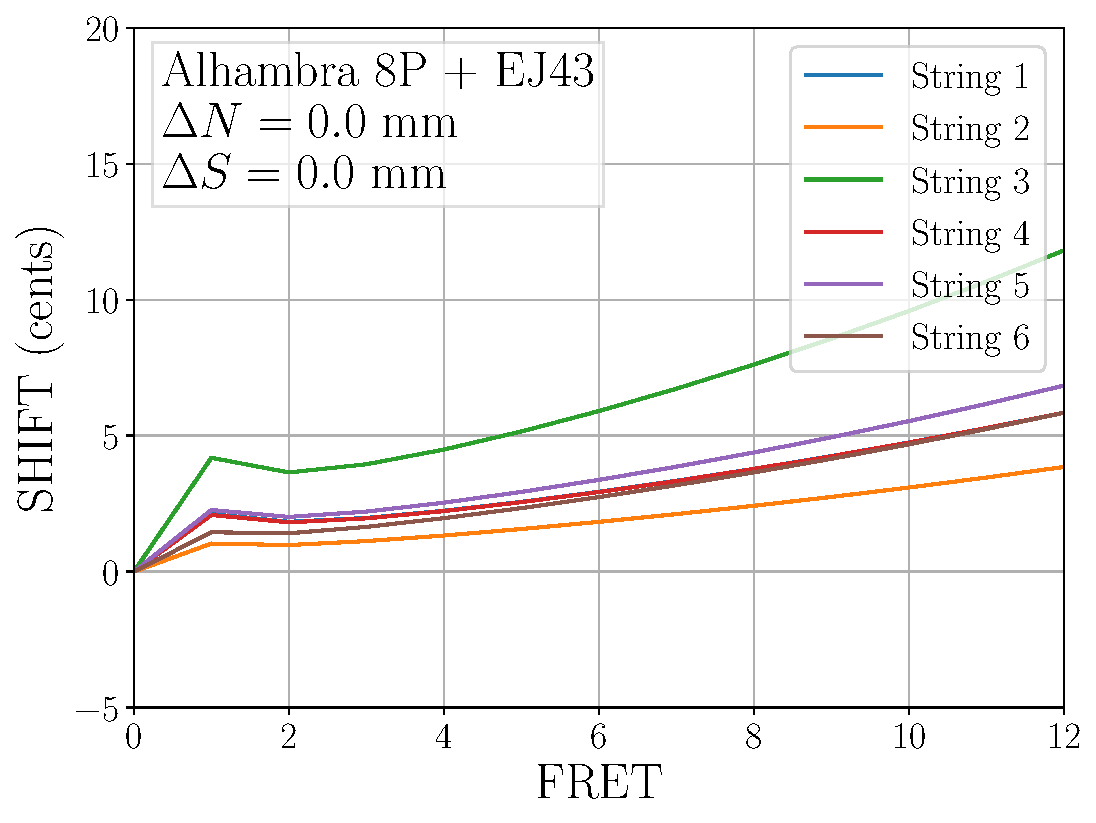
\includegraphics[width=3.25in]{figures/shift_alhambra8p_ej43_null}
   \caption{Uncompensated}
   \label{fig:shift_alhambra8p_ej43_null}
  \end{subfigure}
  \hspace{0.25in}
  \begin{subfigure}[b]{0.45\textwidth}
   \centering
   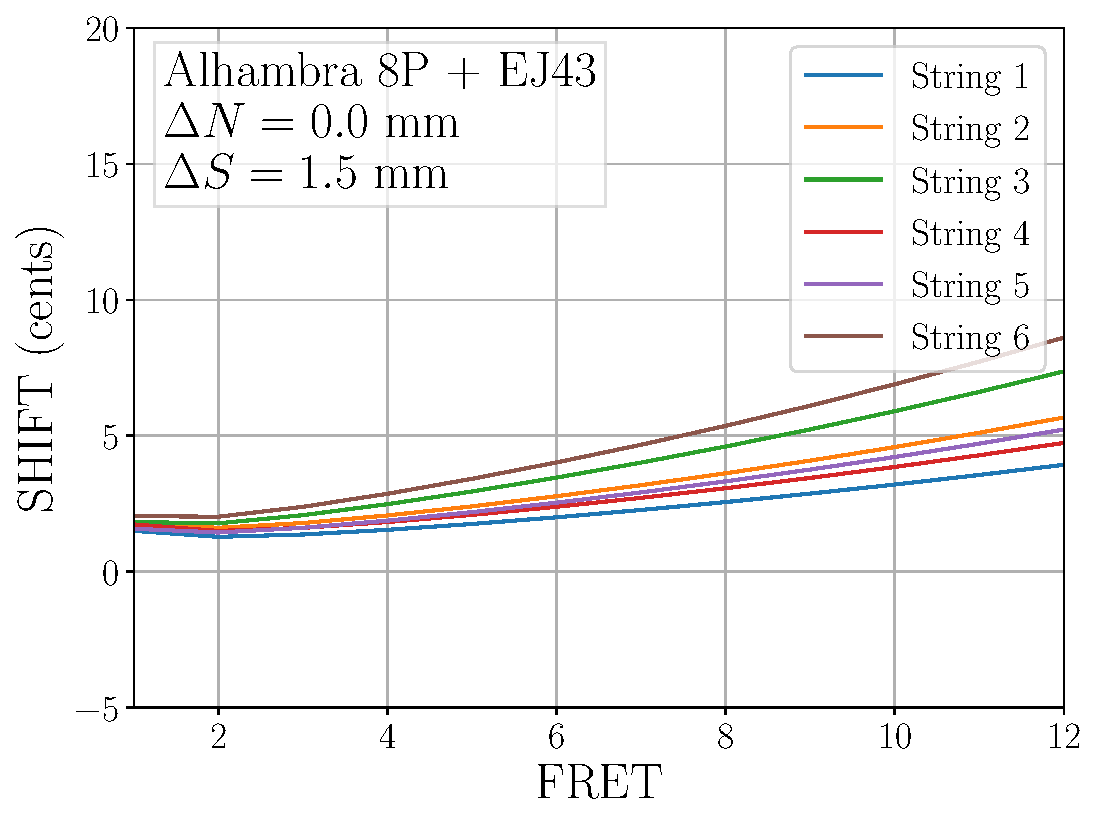
\includegraphics[width=3.25in]{figures/shift_alhambra8p_ej43_factory}
   \caption{Factory guitar}
   \label{fig:shift_alhambra8p_ej43_factory}
  \end{subfigure}
  \par\vspace{0.25in}
  \begin{subfigure}[b]{0.45\textwidth}
   \centering
   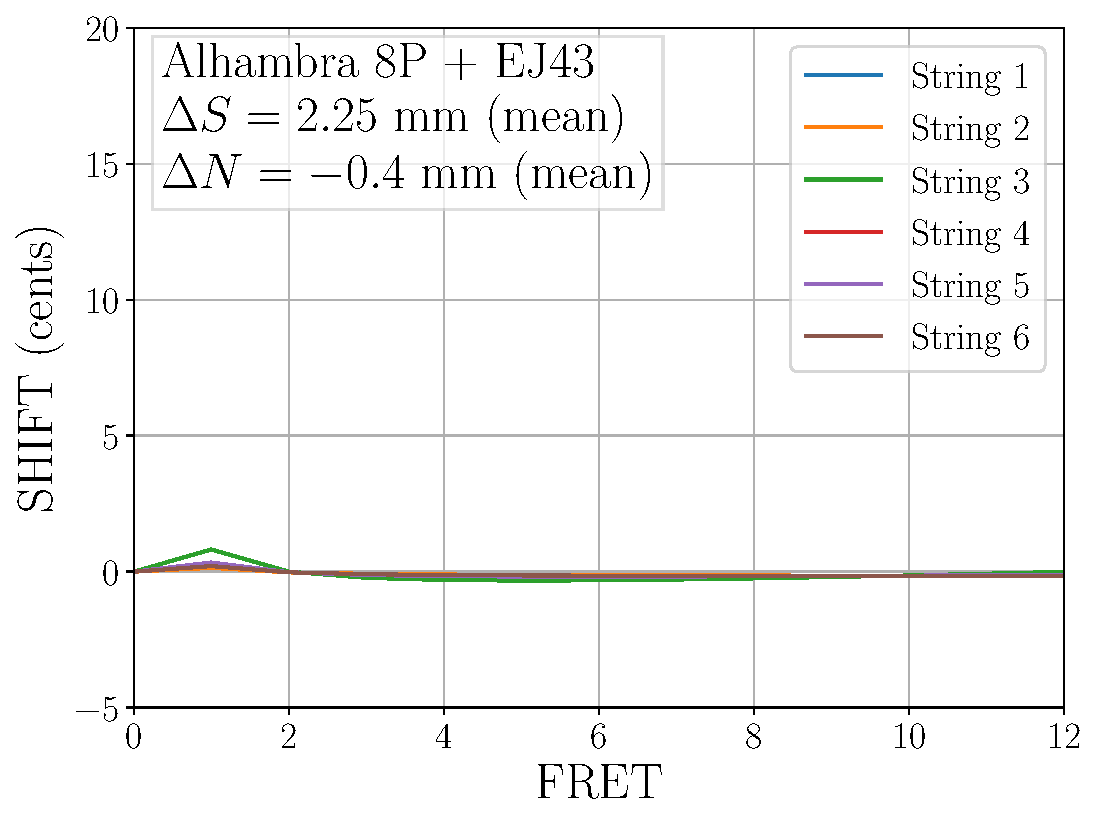
\includegraphics[width=3.25in]{figures/shift_alhambra8p_ej43_full}
   \caption{Full compensation}
   \label{fig:shift_alhambra8p_ej43_full}
  \end{subfigure}
  \hspace{0.25in}
  \begin{subfigure}[b]{0.45\textwidth}
   \centering
   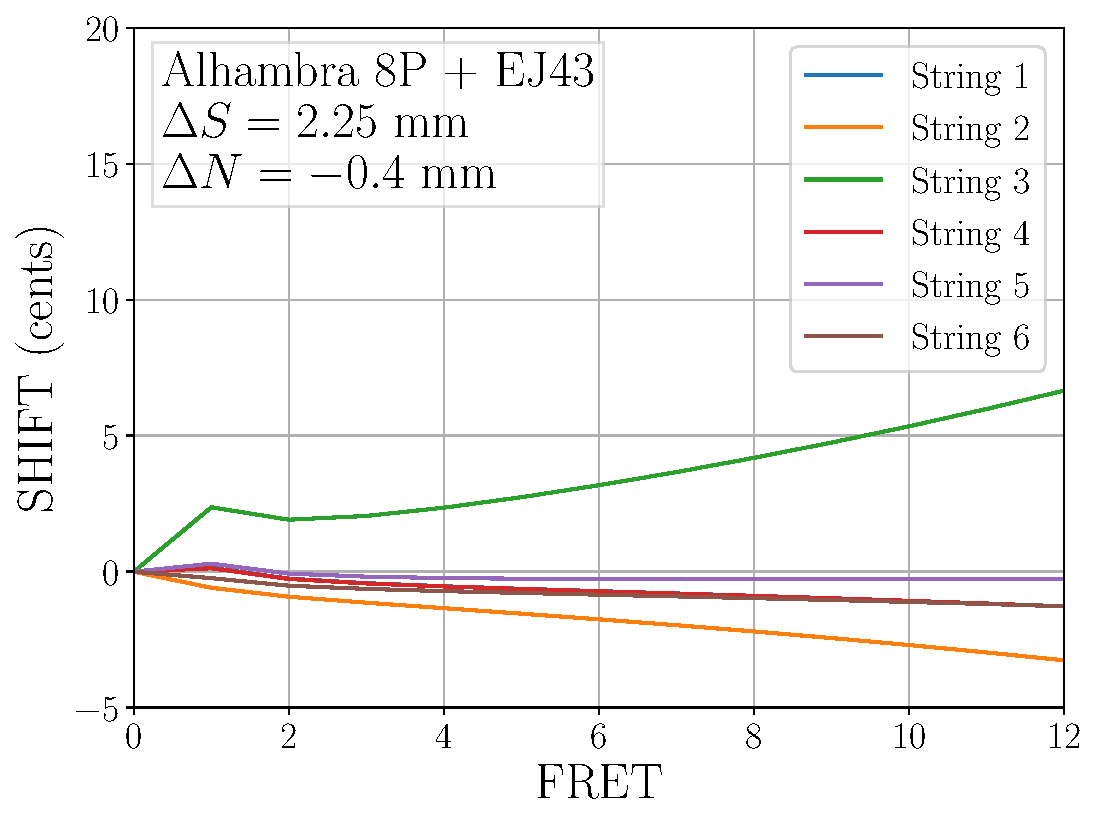
\includegraphics[width=3.25in]{figures/shift_alhambra8p_ej43_mean}
   \caption{Mean compensation}
   \label{fig:shift_alhambra8p_ej43_mean}
  \end{subfigure}
  \caption{\label{fig:compensation_alhambra8p_ej43} Frequency shift (in cents) for an Alhambra 8P guitar with D'Addario Pro-Arte Nylon Classical Guitar Strings -- Light Tension (EJ43). Four different strategies of saddle and nut compensation are illustrated.}
 \end{figure}

 \newpage
 \subsection{Hard Tension}

 \begin{table}[htbp]
  \centering
  \caption{\label{tbl:ej46_ips} String specifications for the D'Addario Pro-Arte Nylon Classical Guitar Strings -- Hard Tension (EJ46). The corresponding scale length is 25.5~inches.}
    \begin{tabular}{lcccc}
    \toprule
    String  & Note  & \multicolumn{1}{l}{Diameter (in)} & \multicolumn{1}{l}{Density (lb/in)} & \multicolumn{1}{l}{Tension (lb)} \\
    \midrule
    J4601 & $E_4$  & 0.0285 & $2.161 \times 10^{-5}$ & 15.8 \\
    J4602 & $B_3$  & 0.0327 & $2.924 \times 10^{-5}$ & 12.0 \\
    J4603 & $G_3$  & 0.0410 & $4.795 \times 10^{-5}$ & 12.4 \\
    J4604 & $D_3$  & 0.0300 & $1.124 \times 10^{-4}$ & 16.3 \\
    J4605 & $A_2$  & 0.0360 & $1.952 \times 10^{-4}$ & 15.9 \\
    J4606 & $E_2$  & 0.0440 & $3.173 \times 10^{-4}$ & 14.5 \\
    \bottomrule
    \end{tabular}%
 \end{table}%

 \begin{table}[htbp]
  \centering
  \caption{\label{tbl:ej46_mks} String specifications for the D'Addario Pro-Arte Nylon Classical Guitar Strings -- Hard Tension (EJ46). The corresponding scale length is 650~mm.}
  \begin{tabular}{ccccc}
\toprule
String &    Note &  Radius (mm) &  Density ($\times 10^{-7}$ kg/mm) &  Tension (N) \\
\midrule
 J4601 & E$_{4}$ &         0.36 &                              3.86 &        70.88 \\
 J4602 & B$_{3}$ &         0.42 &                              5.22 &        53.83 \\
 J4603 & G$_{3}$ &         0.52 &                              8.57 &        55.61 \\
 J4604 & D$_{3}$ &         0.38 &                             20.07 &        73.14 \\
 J4605 & A$_{2}$ &         0.46 &                             34.87 &        71.31 \\
 J4606 & E$_{2}$ &         0.56 &                             56.67 &        65.04 \\
\bottomrule
\end{tabular}


 \end{table}%

 \begin{table}[htbp]
  \centering
  \caption{\label{tbl:ej46_props} Derived physical properties of the D'Addario Pro-Arte Nylon Classical Guitar Strings -- Hard Tension (EJ46). The corresponding scale length is 650 mm.}
  \begin{tabular}{cccccc}
\toprule
String &  $\Delta \nu_{12}$ (cents) &  $R$ ($\times 10^4$) &  $\kappa$ &  $E$ (GPa) &  $B_0$ ($\times 10^{-3}$) \\
\midrule
 J4601 &                          3 &                 12.2 &     139.8 &       24.1 &                       3.3 \\
 J4602 &                          2 &                  6.3 &      71.9 &        7.1 &                       2.7 \\
 J4603 &                         10 &                  5.2 &      59.4 &        3.9 &                       3.1 \\
 J4604 &                          0 &                  6.7 &      76.6 &       12.3 &                       2.6 \\
 J4605 &                          2 &                  3.3 &      37.5 &        4.1 &                       2.2 \\
 J4606 &                          4 &                  4.9 &      55.5 &        3.7 &                       3.2 \\
\bottomrule
\end{tabular}


 \end{table}%

 \begin{table}[htbp]
  \centering
  \caption{\label{tbl:ej46_setbacks} Predicted setbacks for the D'Addario Pro-Arte Nylon Classical Guitar Strings -- Hard Tension (EJ46) on the Alhambra 8P classical guitar.}
  \begin{tabular}{cccccc}
\toprule
String & $\Delta S$ (mm) & $\Delta N$ (mm) & $\overline{\Delta \nu}_\text{rms}$ (cents) \\
\midrule
J4601 & 1.55 & -0.35 & 0.16 \\
J4602 & 1.87 & -0.39 & 0.18 \\
J4603 & 2.39 & -0.42 & 0.19 \\
J4604 & 1.59 & -0.34 & 0.16 \\
J4605 & 1.93 & -0.36 & 0.17 \\
J4606 & 2.40 & -0.38 & 0.18 \\
\bottomrule
\end{tabular}


 \end{table}%

 \begin{figure}
  \centering
  \begin{subfigure}[b]{0.45\textwidth}
   \centering
   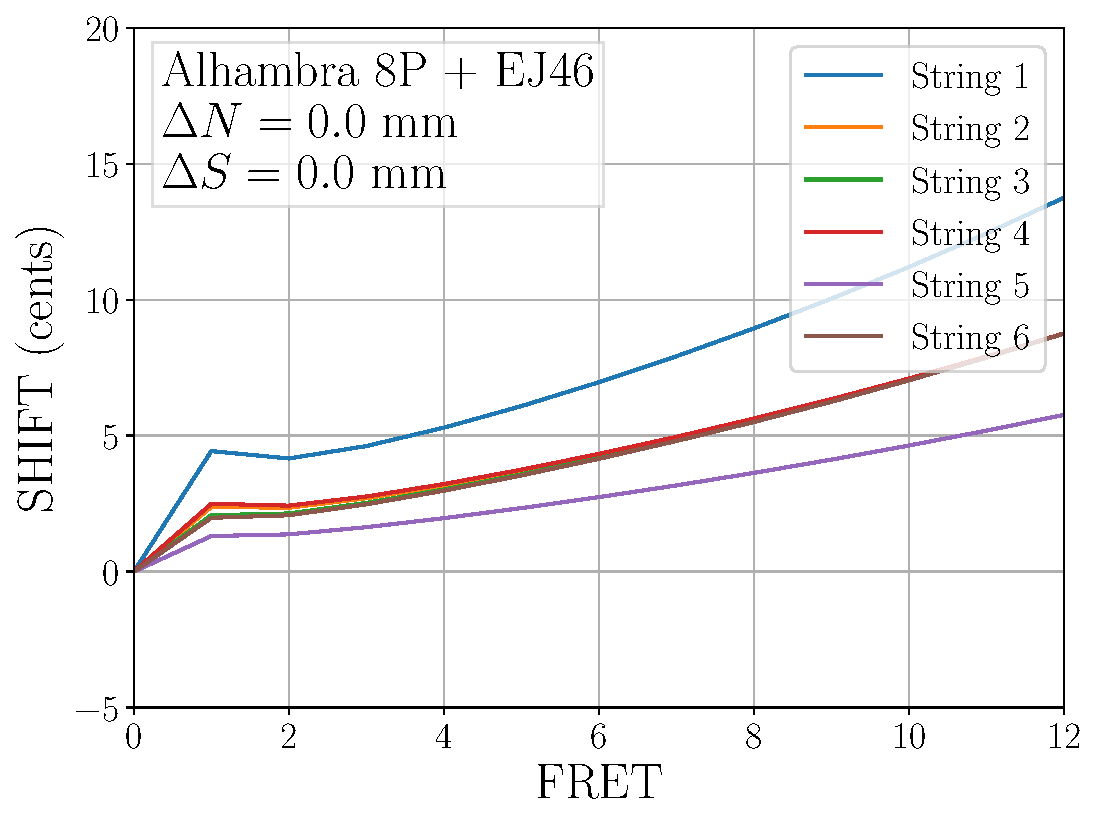
\includegraphics[width=3.25in]{figures/shift_alhambra8p_ej46_null}
   \caption{Uncompensated}
   \label{fig:shift_alhambra8p_ej46_null}
  \end{subfigure}
  \hspace{0.25in}
  \begin{subfigure}[b]{0.45\textwidth}
   \centering
   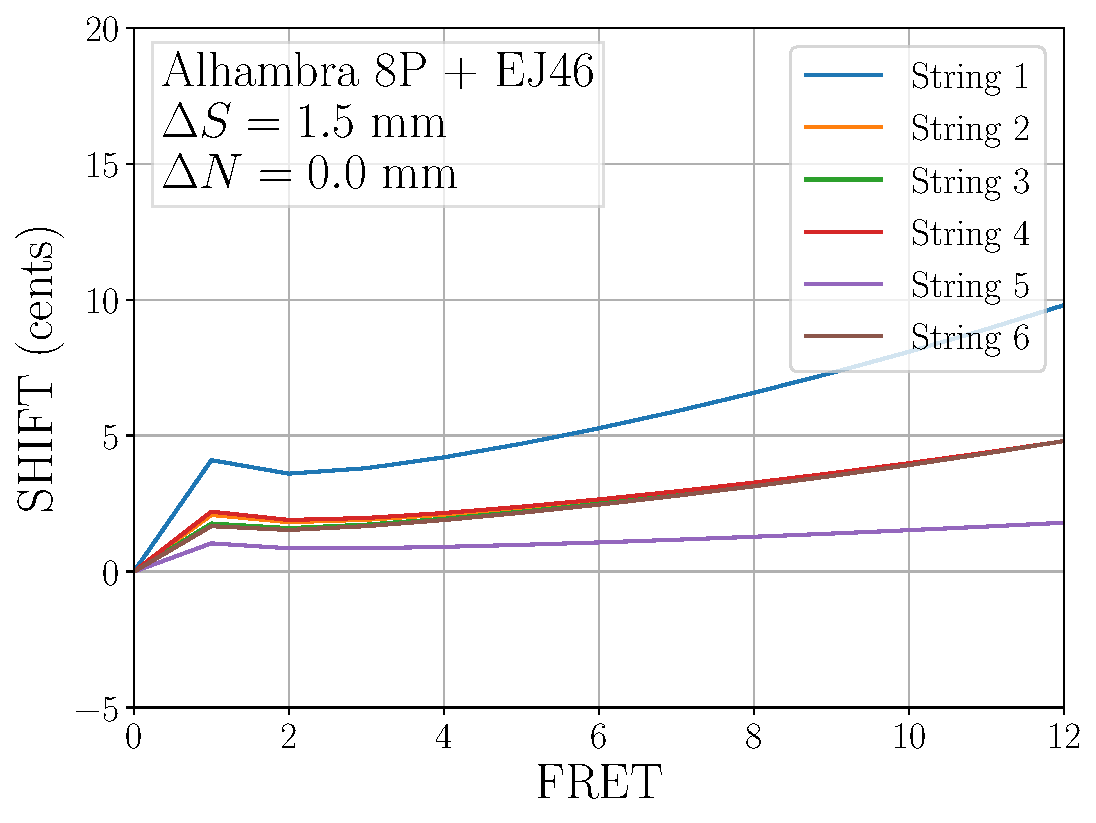
\includegraphics[width=3.25in]{figures/shift_alhambra8p_ej46_factory}
   \caption{Factory guitar}
   \label{fig:shift_alhambra8p_ej46_factory}
  \end{subfigure}
  \par\vspace{0.25in}
  \begin{subfigure}[b]{0.45\textwidth}
   \centering
   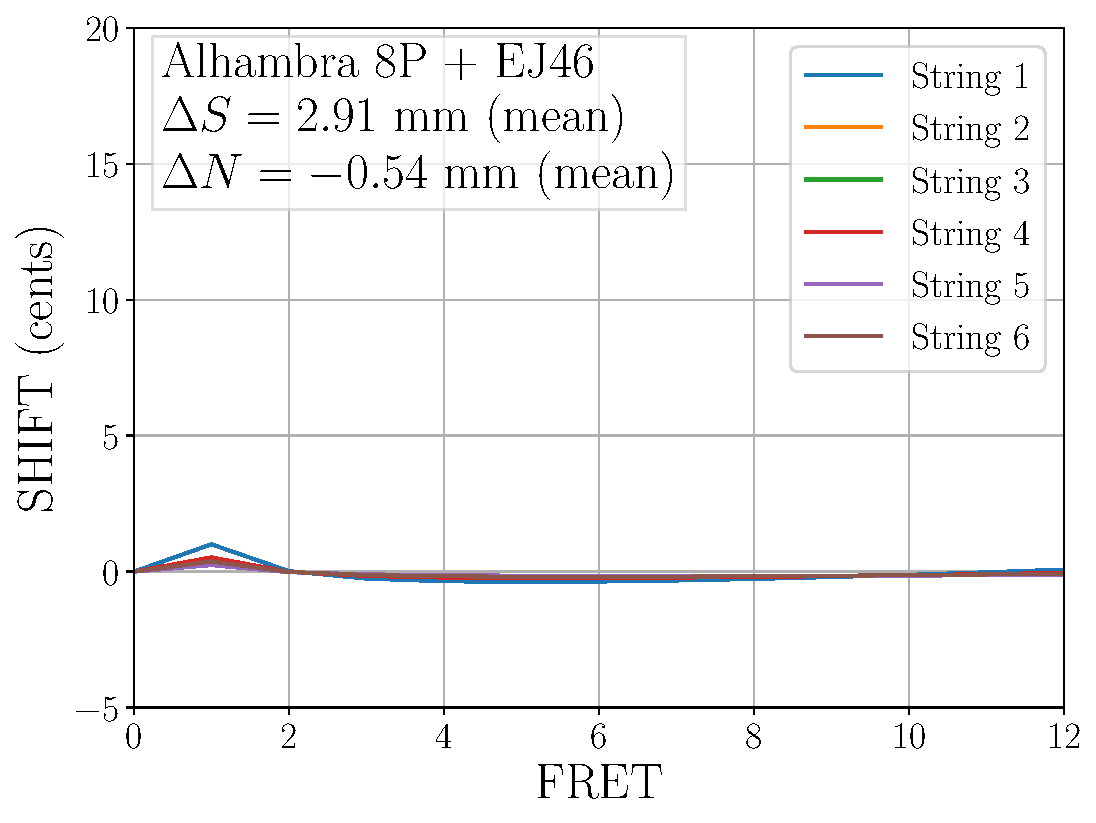
\includegraphics[width=3.25in]{figures/shift_alhambra8p_ej46_full}
   \caption{Full compensation}
   \label{fig:shift_alhambra8p_ej46_full}
  \end{subfigure}
  \hspace{0.25in}
  \begin{subfigure}[b]{0.45\textwidth}
   \centering
   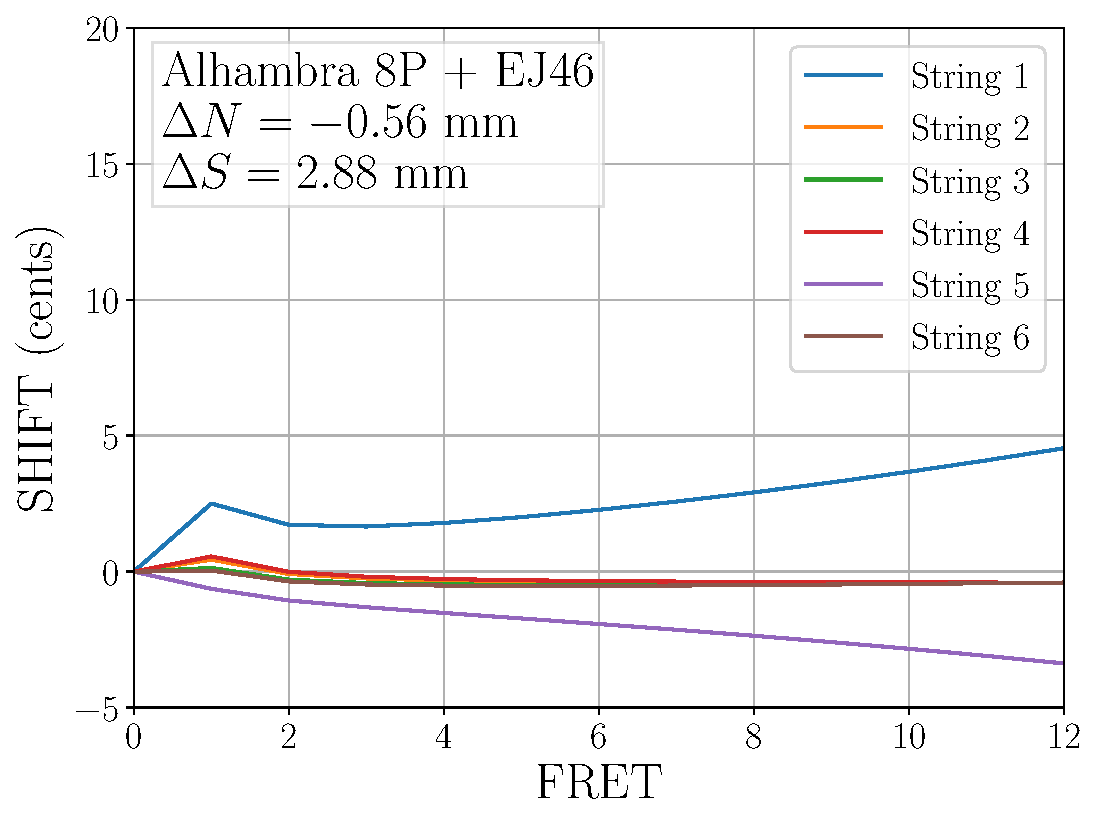
\includegraphics[width=3.25in]{figures/shift_alhambra8p_ej46_mean}
   \caption{Mean compensation}
   \label{fig:shift_alhambra8p_ej46_mean}
  \end{subfigure}
  \caption{\label{fig:compensation_alhambra8p_ej46} Frequency shift (in cents) for an Alhambra 8P guitar with D'Addario Pro-Arte Nylon Classical Guitar Strings -- Hard Tension (EJ46). Four different strategies of saddle and nut compensation are illustrated.}
 \end{figure}

 \newpage
 \subsection{Extra Hard Tension}

 \begin{table}[htbp]
  \centering
  \caption{\label{tbl:ej44_ips} String specifications for the D'Addario Pro-Arte Nylon Classical Guitar Strings -- Extra Hard Tension (EJ44). The corresponding scale length is 25.5~inches.}
    \begin{tabular}{lcccc}
    \toprule
    String  & Note  & \multicolumn{1}{l}{Diameter (in)} & \multicolumn{1}{l}{Density (lb/in)} & \multicolumn{1}{l}{Tension (lb)} \\
    \midrule
    J4401 & $E_4$  & 0.0290 & $2.243 \times 10^{-5}$ & 16.4 \\
    J4402 & $B_3$  & 0.0333 & $3.046 \times 10^{-5}$ & 12.5 \\
    J4403 & $G_3$  & 0.0416 & $4.989 \times 10^{-5}$ & 12.9 \\
    J4404 & $D_3$  & 0.0300 & $1.124 \times 10^{-4}$ & 16.3 \\
    J4405 & $A_2$  & 0.0360 & $1.952 \times 10^{-4}$ & 15.9 \\
    J4406 & $E_2$  & 0.0450 & $3.435 \times 10^{-4}$ & 15.7 \\
    \bottomrule
    \end{tabular}%
 \end{table}%

 \begin{table}[htbp]
  \centering
  \caption{\label{tbl:ej44_mks} String specifications for the D'Addario Pro-Arte Nylon Classical Guitar Strings -- Extra Hard Tension (EJ44). The corresponding scale length is 650~mm.}
  \begin{tabular}{ccccc}
\toprule
String &   Note &  Radius (mm) &  Density ($\times 10^{-7}$ kg/mm) &  Tension (N) \\
\midrule
 J4401 &  $E_4$ &         0.37 &                              4.01 &        73.57 \\
 J4402 &  $B_3$ &         0.42 &                              5.44 &        56.07 \\
 J4403 &  $G_3$ &         0.53 &                              8.91 &        57.86 \\
 J4404 &  $D_3$ &         0.38 &                             20.07 &        73.14 \\
 J4405 &  $A_2$ &         0.46 &                             34.87 &        71.31 \\
 J4406 &  $E_2$ &         0.57 &                             61.36 &        70.42 \\
\bottomrule
\end{tabular}


 \end{table}%

 \begin{table}[htbp]
  \centering
  \caption{\label{tbl:ej44_props} Derived physical properties of the D'Addario Pro-Arte Nylon Classical Guitar Strings -- Extra Hard Tension (EJ44). The corresponding scale length is 650 mm.}
  \begin{tabular}{cccccc}
\toprule
String &  $\Delta \nu_{12}$ (cents) &  $R$ ($\times 10^4$) &  $\kappa$ &  $E$ (GPa) &  $B_0$ ($\times 10^{-3}$) \\
\midrule
 J4401 &                          3 &                  4.0 &      45.4 &        7.8 &                       1.9 \\
 J4402 &                          2 &                  8.1 &      92.7 &        9.3 &                       3.1 \\
 J4403 &                         10 &                  9.5 &     108.2 &        7.1 &                       4.2 \\
 J4404 &                          0 &                  6.7 &      76.6 &       12.3 &                       2.6 \\
 J4405 &                          2 &                  3.3 &      37.5 &        4.1 &                       2.2 \\
 J4406 &                          4 &                  4.8 &      54.3 &        3.7 &                       3.2 \\
\bottomrule
\end{tabular}


 \end{table}%

 \begin{table}[htbp]
  \centering
  \caption{\label{tbl:ej44_setbacks} Predicted setbacks for the D'Addario Pro-Arte Nylon Classical Guitar Strings -- Extra Hard Tension (EJ44) on the Alhambra 8P classical guitar.}
  \begin{tabular}{cccc}
\toprule
String &  $\Delta S$ (mm) &  $\Delta N$ (mm) &  $\overline{\Delta \nu}_\text{rms}$ (cents) \\
\midrule
 J4401 &             1.89 &            -0.34 &                                        0.16 \\
 J4402 &             3.38 &            -0.69 &                                        0.26 \\
 J4403 &             4.39 &            -0.80 &                                        0.30 \\
 J4404 &             2.76 &            -0.57 &                                        0.22 \\
 J4405 &             1.95 &            -0.28 &                                        0.15 \\
 J4406 &             2.94 &            -0.40 &                                        0.17 \\
\bottomrule
\end{tabular}


 \end{table}%

 \begin{figure}
  \centering
  \begin{subfigure}[b]{0.45\textwidth}
   \centering
   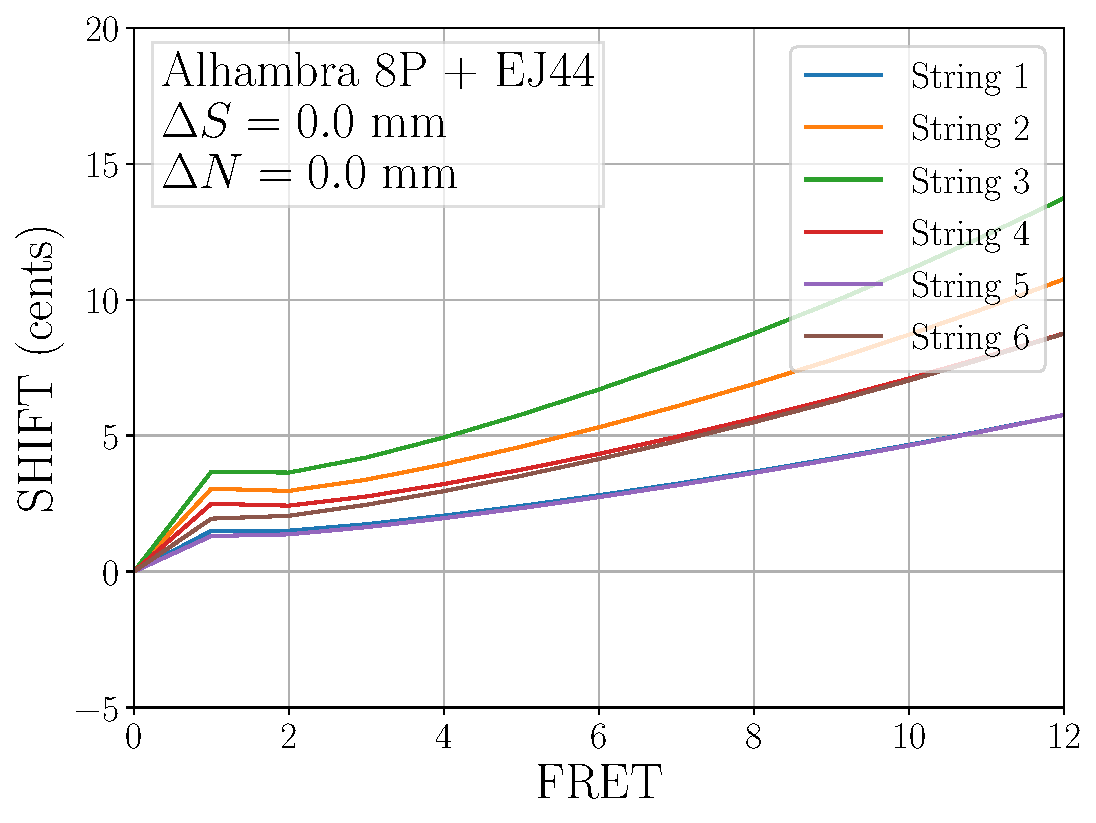
\includegraphics[width=3.25in]{figures/shift_alhambra8p_ej44_null}
   \caption{Uncompensated}
   \label{fig:shift_alhambra8p_ej44_null}
  \end{subfigure}
  \hspace{0.25in}
  \begin{subfigure}[b]{0.45\textwidth}
   \centering
   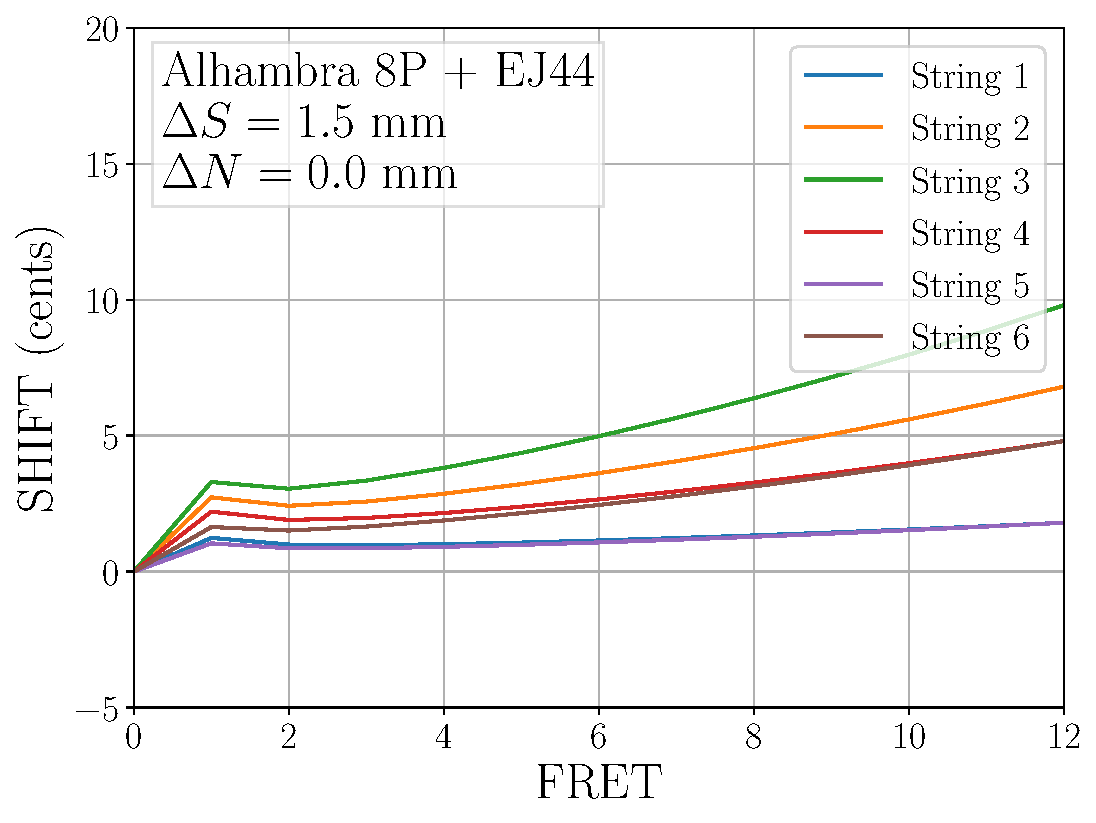
\includegraphics[width=3.25in]{figures/shift_alhambra8p_ej44_factory}
   \caption{Factory guitar}
   \label{fig:shift_alhambra8p_ej44_factory}
  \end{subfigure}
  \par\vspace{0.25in}
  \begin{subfigure}[b]{0.45\textwidth}
   \centering
   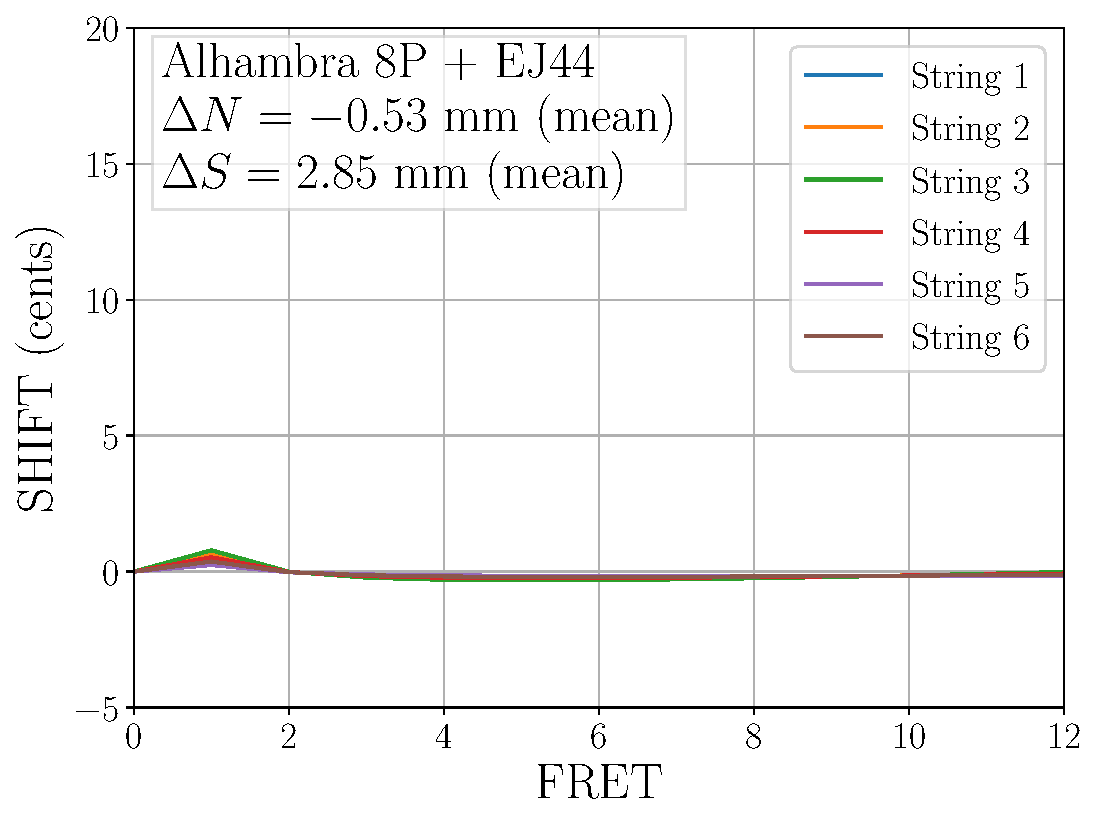
\includegraphics[width=3.25in]{figures/shift_alhambra8p_ej44_full}
   \caption{Full compensation}
   \label{fig:shift_alhambra8p_ej44_full}
  \end{subfigure}
  \hspace{0.25in}
  \begin{subfigure}[b]{0.45\textwidth}
   \centering
   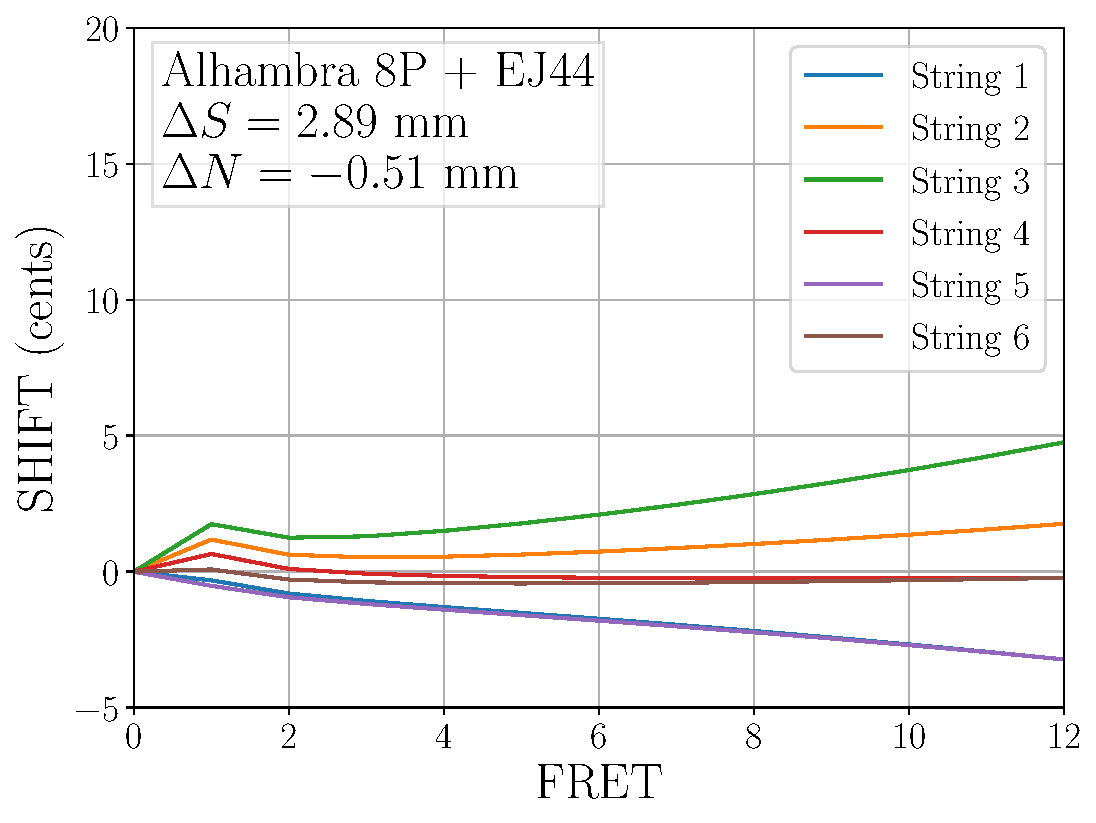
\includegraphics[width=3.25in]{figures/shift_alhambra8p_ej44_mean}
   \caption{Mean compensation}
   \label{fig:shift_alhambra8p_ej44_mean}
  \end{subfigure}
  \caption{\label{fig:compensation_alhambra8p_ej44} Frequency shift (in cents) for an Alhambra 8P guitar with D'Addario Pro-Arte Nylon Classical Guitar Strings -- Extra Hard Tension (EJ44). Four different strategies of saddle and nut compensation are illustrated.}
 \end{figure}
